\documentclass[compsoc]{IEEEtran}
\usepackage{graphicx}
\usepackage{amsmath}
\usepackage{authblk}
\usepackage[english]{babel}
\usepackage{blindtext}
%\usepackage[ruled,vlined,linesnumbered]{algorithm2e}
%\usepackage{algorithmic,float}
\usepackage{setspace}
\usepackage{amsfonts}
%\usepackage{hyperref}
\graphicspath{ {../images/} }
\usepackage{subfig}
\usepackage{fontspec}
\usepackage{listings}
\usepackage{amsmath}
\usepackage{mathabx}
\usepackage[bottom]{footmisc}
\newfontfamily\listingsfont[Scale=.7]{inconsolata}\usepackage[font=footnotesize,labelfont=bf]{caption}
%\captionsetup[algorithm2e]{font=footnotesize}
\usepackage[table,xcdraw]{xcolor}
\usepackage[utf8]{inputenc}
\title{Assignment: Transfer Learning on Intel Image Classification}
\author{David Bertoldi -- 735213 \\ email: d.bertoldi@campus.unimib.it}
\affil{Department of Informatics, Systems and Communication}
\affil{University of Milano-Bicocca}
\date{October 2022}


\begin{document}

\maketitle 



\section{Inspecting the data}\label{sec:insp}
The MNIST dataset contains $70\,000$ images of handwritten digits ($0$ to $9$) that have been size-normalized and centered in a square grid of pixels. Each image is a $28 \times 28$ array of floating-point numbers representing grayscale intensities ranging from $0$ (black) to $255$ (white). \par
The labels consist of a vector of values, corresponding to the digit classification categories $0$ through $9$. \par
The dataset is already divided into training and test sets, respectively with $60\,000$ and $10\,000$ samples. \par

Figure \ref{fig:data} shows an 10 entries of the training dataset.

\begin{figure}[ht!]
\centering                                                                        
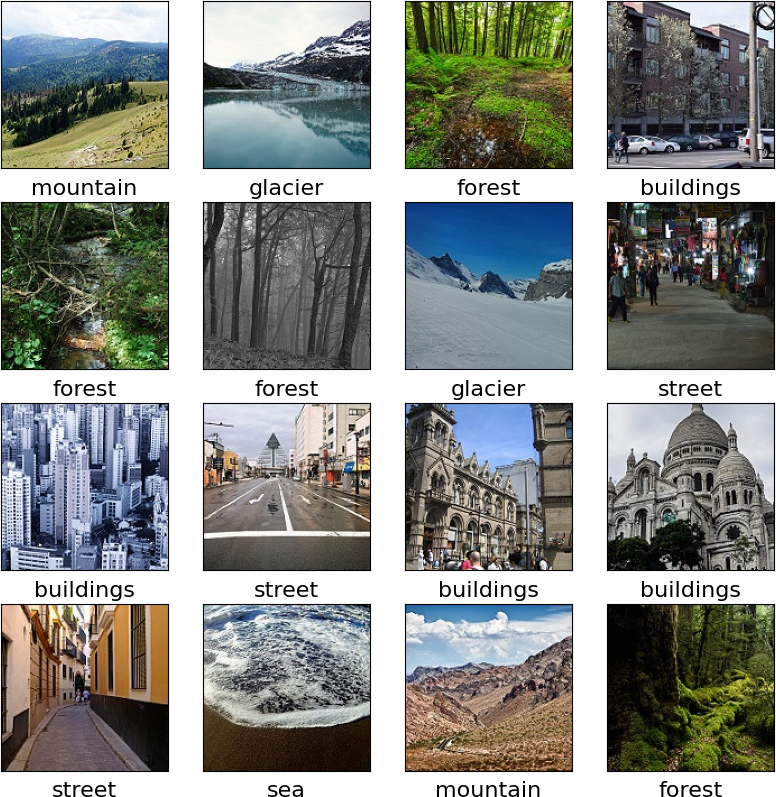
\includegraphics[width=2.5in]{../images/samples.png}
\captionsetup{justification=centering}                                                                                         
\caption{The first 10 samples of the train dataset}
\label{fig:data}                                                                                                                               
\end{figure}




The training population presents a distribution with mean $\mu = 6\,000$ and standard deviation $\sigma \simeq 340$ and thus we didn't notice any important unbalance in the data. For this reason we assumed the data followed a distribution $X \sim U(\mu, \sigma)$ and no data augmentation on less populated classes was taken into account. Figure \ref{fig:hist} shows the data distribution for both training and test datasets.

\begin{figure}[ht!]
\centering                                                                        
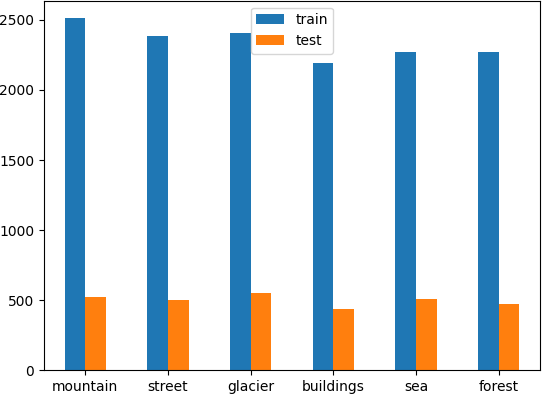
\includegraphics[width=3.5in]{../images/data.png}
\captionsetup{justification=centering}                                                                                         
\caption{Histogram of the frequency of samples in the dataset}
\label{fig:hist}                                                                                                                               
\end{figure}

\section{Preparing the data}
Before training a CNN using this images, encoded in $28\times28$ matrices with values from $0$ to $255$, we rescaled each value in the continuous interval $[0, 1]$ and expanded the dimensionality of the matrix to $1 \times 28 \times 28$. This encoding will be used in every section of this work: small values increase the efficiency in the calculations and \texttt{Conv2D} requires an additional dimension that describes the channels (in this case just one for the grayscale).


\subsection{Data split}
As noted in section \ref{sec:insp}, the dataset is divided into training and test samples. A set of items to be used for validation is missing and thus
is retrieved from the training set: $15\%$ of the images are randomly used for validation (along with their labels) for a total of $9\,000$ samples. \par
The labels were encoded in one-hot vectors so that the $1$s were set in the index representing the numerical class. \par

\section{Building the network and training}
The aim of this section is to describe a CNN with less than $10\,000$ parameters that is able to classify
with the highest possible level of test categorical accuracy the numbers from the dataset in $10$ epochs and batches of $128$ samples. 

\subsection{The network}
The CNN presents a typical architecure formed by convolutional layers followed by pooling layers and ending with dense layers. \par
In particular there are 2 convulutional layers covering the whole $28 \times 28$ image, formed by eight $3 \times 3$ filters, for a total dimension of $28 \times 28 \times 8$. These two layers are followed by a \emph{max pooling} layer that halves the the widht and height of the outcoming activation map. For this problem we tested both \emph{max pooling} and \emph{average pooling}; the first one performed slighty better ($+0.2\%$ in test categorical accuracy): usually \emph{average pooling} smooths out the image and has harder times to identify sharp features while \emph{max pooling} chooses only the brightest pixels of the image that are in this case the ones defining the handwritten digit. Although we noticed a slighty improvement using \emph{max pooling}, the images are too small to actually benefit from the methods' differences. \par
The structure continues with another one convolutional layer aligned with the 2D spatiality of the last pooling layer but doubled in the depth, that is $7 \times 7 \times 16$. The convolutional layer is reduced in spatiality by another \emph{max pooling layer} $7 \times 7 \times 16$ and flattened in a 1D array of $784$. The input flows to the output layer activated by \emph{Softmax} function. Figure \ref{fig:cnn} summarizes the entire architecture and Table \ref{tab:count} highlights the number of parameters in each layer.



\begin{table}[ht!]
\begin{tabular}{|ll|l|}
\hline
\rowcolor[HTML]{3166FF} 
\multicolumn{1}{|l|}{\cellcolor[HTML]{3166FF}{\color[HTML]{FFFFFF} \textbf{Layer}}} & {\color[HTML]{FFFFFF} \textbf{Size}} & {\color[HTML]{FFFFFF} \textbf{Parameters}} \\ \hline
\multicolumn{1}{|l|}{input}                                                         & $28\times28\times1$                          &   $0$                                             \\ \hline
\multicolumn{1}{|l|}{Conv2D-1}                                                      & $28\times28\times8$                           &  $(3\cdot3\cdot1+1)\cdot8 = 80$                                            \\ \hline
\multicolumn{1}{|l|}{Conv2D-2}                                                      & $28\times28\times8$                            &  $(3\cdot3\cdot8 + 1)\cdot8 = 584$                                            \\ \hline
\multicolumn{1}{|l|}{MaxPool-1}                                                     & $14\times14\times8$                            &  $0$                                            \\ \hline
\multicolumn{1}{|l|}{Conv2D-3}                                                      & $14\times14\times16$                            & $(3\cdot3\cdot8 + 1)\cdot16 = 1\,168$                                            \\ \hline
\multicolumn{1}{|l|}{MaxPool-2}                                                      & $7\times7\times16$                            & $0$                                            \\ \hline
\multicolumn{1}{|l|}{Flatten}                                                       & $1\times1\times784$                            & $0$                                            \\ \hline
\multicolumn{1}{|l|}{Dense}                                                         & $1\times1\times10$                            & $(784 + 1)\cdot10 = 7\,850$                                            \\ \hline
\multicolumn{2}{|l|}{\textbf{Total}}                                                                                       &       $9\,682$                                     \\ \hline
\end{tabular}
\caption{Summary of the layers' dimensions and count of the parameters for each layer}
\label{tab:count}
\end{table}



\begin{figure}[ht!]
\centering                                                                        
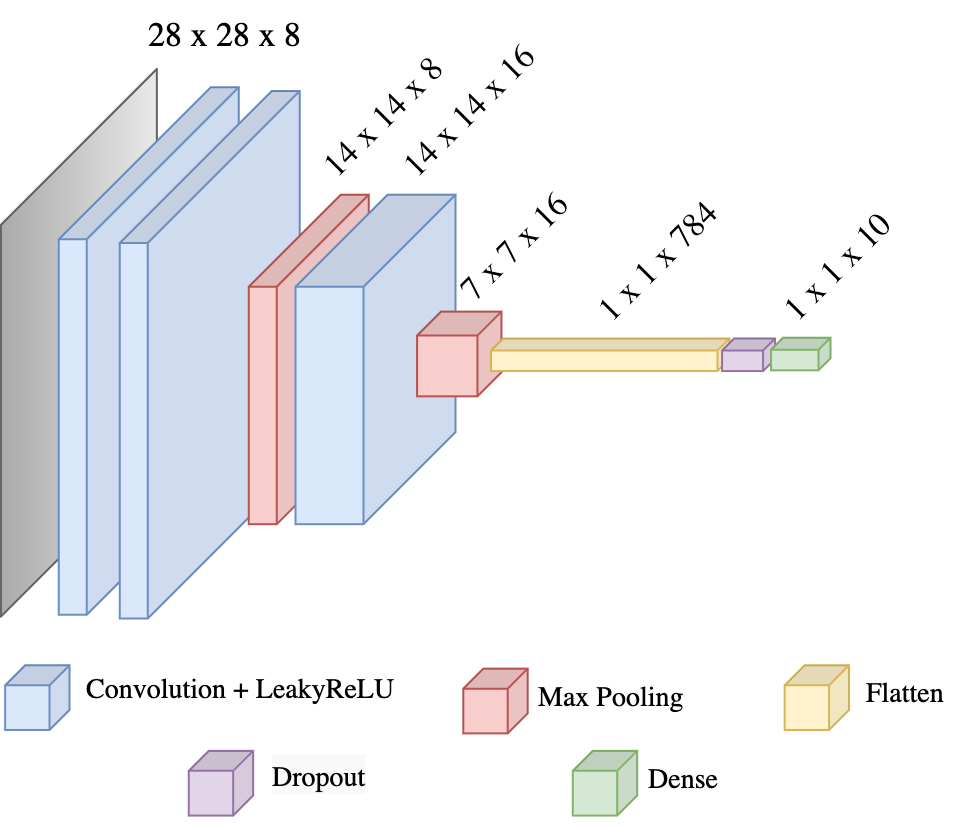
\includegraphics[width=3.5in]{cnn.png}
\captionsetup{justification=centering}                                                                                         
\caption{Architecture of the CNN}
\label{fig:cnn}                                                                                                                               
\end{figure}

On the structure, we tried less deeper convolitional layers (starting from $28\times28\times4$ and then scaling to $14\times14\times8$) but the overall categorical accuracy dropped by $0.8\%$.

About the convulutional layers, Tensorflow allows to specify the padding: no padding and padding with zeroes. The first one would had reduced the spatiality of each layer by $1$, the second one preserves the dimensions by putting evenly $0$s on the margins. Adding $0$s with this particular dataset is not an issue, because most of the images (if not all of them) do not contain information along the margins.
We benchmarked the performances of both methods and we noticed that the zero padding gave an higher validation categorical accuracy of $+0.3\%$.




\subsection{Training}
The choice of the optimizer was among \emph{RMSProp} and \emph{Adam}. 
None of them have shown signs of getting stuck in local minimum regions but \emph{Adam} performed better overall, with $+0.9\%$ on test accuracy. \par

The only regularization used is the \emph{dropout} technique applied to the flattened layer with a rate of $10\%$. This allowed the model to not overifit too much and generalize better the problem. The choice of the probability to drop out a neuron is based on the chart in Figure \ref{fig:drop} where we moved the rate
from $0\%$ to $90\%$ and logged the results for training, validation and test categorical accuracy.


\begin{figure}[ht!]
\centering                                                                        
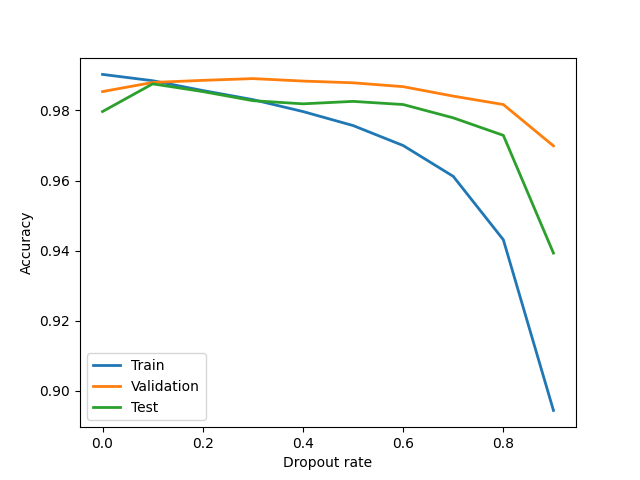
\includegraphics[width=3.5in]{drop.png}
\captionsetup{justification=centering}                                                                                         
\caption{Loss}
\label{fig:drop}                                                                                                                               
\end{figure}

We chose a drop rate of $10\%$ because it maximized the test categorical accuracy, raised the validation categorical accuracy and introduced a noticeable amount of underfitting, which decreased the training categorical accuracy. \footnote{This is the best configuration with 10 epochs and batch size of 128. We noticed better results with higher drop rate ($40\%$) with more epochs, limited by \emph{early stopping} techniques, and 256 batch size: this configuration produced a $98.92\%$ in test accuracy.}
\par

The behaviour of the model during the training phase is described in the plots of the loss and categorical accuracy in 
Figure \ref{fig:loss} and Figure \ref{fig:acc}. 

\begin{figure}[ht!]
\centering                                                                        
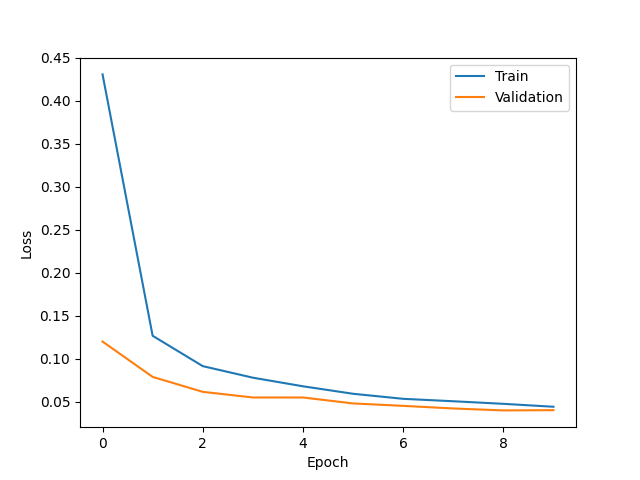
\includegraphics[width=3.5in]{loss.png}
\captionsetup{justification=centering}                                                                                         
\caption{Loss}
\label{fig:loss}                                                                                                                               
\end{figure}


\begin{figure}[ht!]
\centering                                                                        
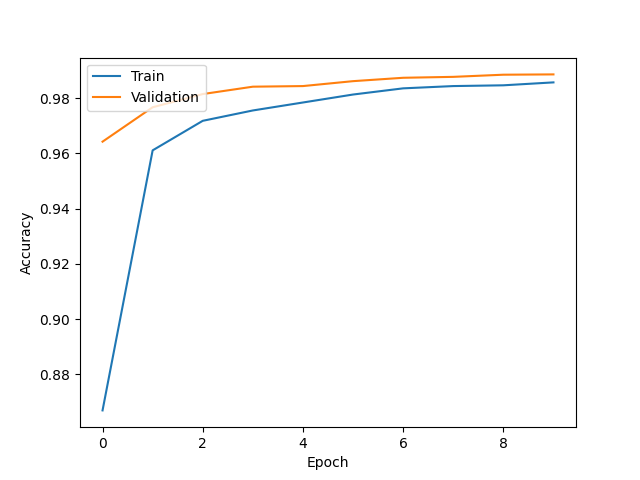
\includegraphics[width=3.5in]{acc.png}
\captionsetup{justification=centering}                                                                                         
\caption{Categorical accuracy}
\label{fig:acc}                                                                                                                               
\end{figure}


The validation loss was always lower than the training loss. This is effect is caused by the \emph{dropout} because it penalizes model variance by randomly removing neurons from the flatten layer only during the training; the models underfitted and since \emph{dropout} is disabled during the validation we had lower validation loss. The same for the categorical accuracy, being higher during validation.\par
The best training and validation categorical accuracy reached in this configuration were $98.57\%$ and $98.86\%$ respectively, using \emph{Adam} with learning rate of $10^{-3}$.


\subsection{Evaluation}
We tested the quality of the model's predictions using the provided test dataset, applying very same transormations on the images used for the training.
The categorical accuracy 
over the test set reached $98.65\%$ and can be analyzed with the help of the confusion matrix (Figure \ref{fig:cm}). 

\begin{figure}[ht!]
\centering                                                                        
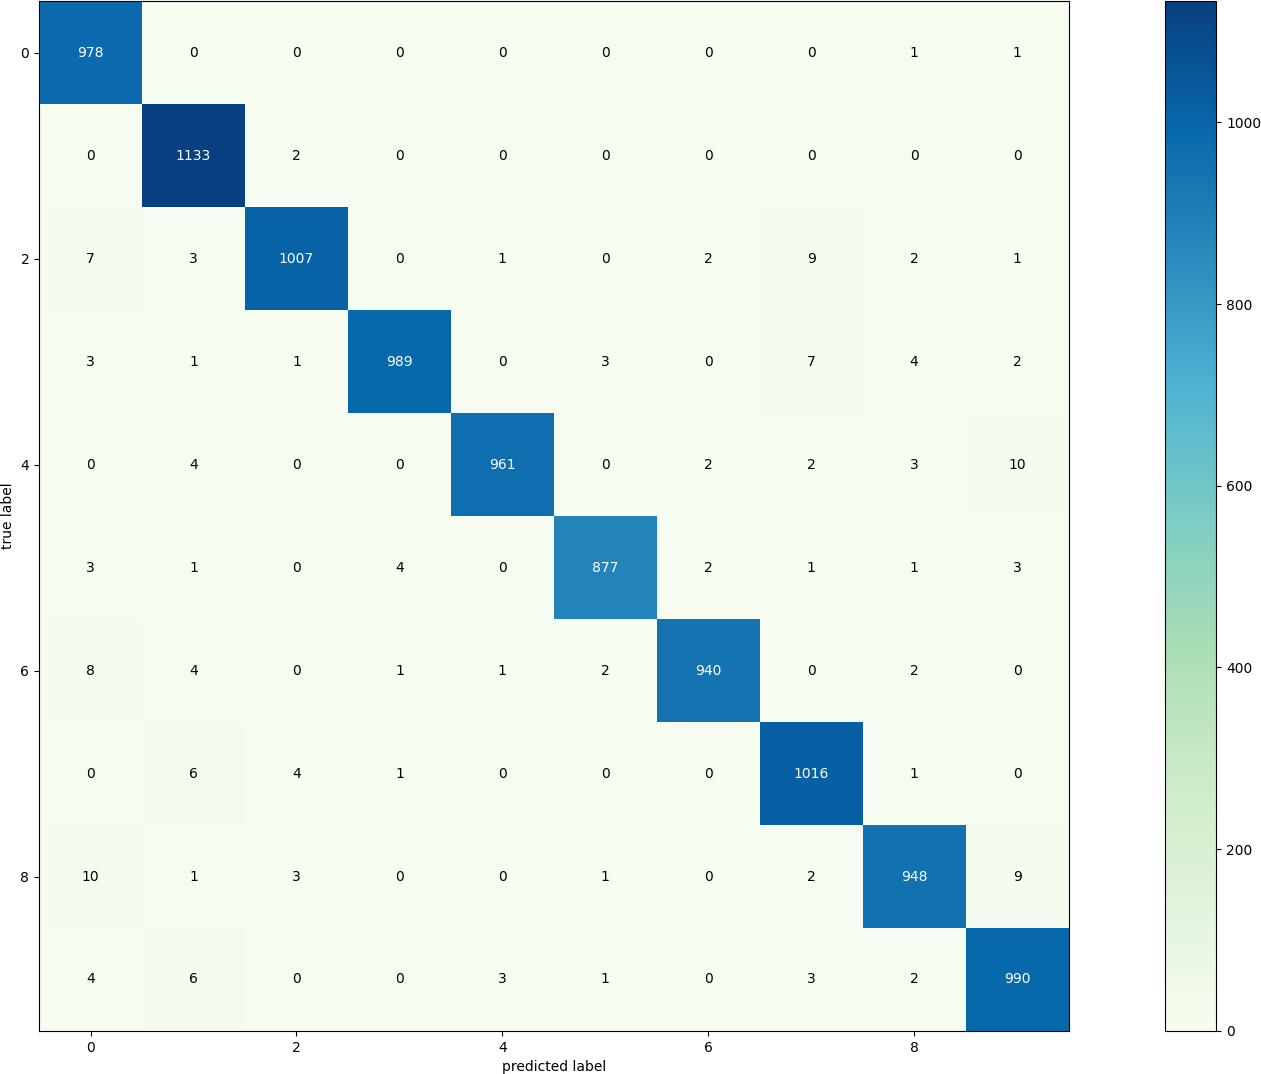
\includegraphics[width=3.5in]{cm2.png}
\captionsetup{justification=centering}                                                                                         
\caption{Confusion matrix over the test data}
\label{fig:cm}                                                                                                                               
\end{figure}

We noticed that the model confused the $0.9\%$ of the $4$s with a $9$: this can be explained by the fact that the two digits have similar forms, in particular when
the $4$ is written quicky and in its \emph{"closed form"}. Apart from these cases, that have a realitively low impact, the model gave really good results.\par

\section{Implementations}
The training of the model can be started with \texttt{trainer.py}. It generates the needed images for the project in \texttt{./images/}
a model checkpoint (hdf5 file) in the working directory. The validation can be performed with \texttt{eval.py} and requires a valid hdf5 file produced by the trainer.\par


\section{Conclusions}
In this work we trained a CNN with less than $10\,000$ parameters, achieving the best test categorical accuracy with $10$ epochs and $128$ elements per batch. We tested an architecure with two sections containing convolutional and pooling layers and ending with a dense ouput, benchmarking different dimensions and applying different rate of drop out. The CNN requires a significative lower number of parameters compared to a dense FNN, achieving better results. The application of local filters (or kernels) helped the model to better recognize sharp features in the images with a very low number of epochs.

\end{document}









